\section{Related Works}
\label{ch:relate}

% - 讨论 client-side 的 clickstream 为什么值得研究,比较服务端搜集的 clickstream 产生的明显变化是什么。
% - 讨论现有的 client-side clickstream 研究分别是针对什么方向的,他们的结论主要是什么,都有什么样的改进空间。
% - 以前的 clickstream 只有类别级的分配模型,通过人工设计某个特定网站的马尔科夫模型来学习用户在不同类别之间的跳转概率。但当变为客户端后,数据变得更加充分,用户在一段时间内可能不局限于某个特定的网站,同时可能被其他网站干扰。

In this chapter, we discuss the former research that releats to our work, including
the existing approaches to clickstream behavior modeling, the evolution of information 
behavior theory regarding how it adapts to our digital world, as well as the 
most related recent advances regarding sequence learning.

\subsection{Clickstream Behavior Modeling}

Clickstream behavior research can be traced back to the year when the word ``clickstream''
was invented. Eearly clickstream behavior research studied the navigational behavior
of user \cite{mandese1995clickstreams, brodwin1995} and 
they binary classified clickstream based on the degree of linearity.

More recently, 


% - 这一篇是第一篇 clientside clickstream 的研究:Nils Kammenhuber, Julia Luxenburger, Anja Feldmann, and Gerhard Weikum. 2006. Web search clickstreams. In Proceedings of the 6th ACM SIGCOMM conference on Internet measurement (IMC '06). ACM, New York, NY, USA, 245-250.

% 关于时间的研究
% @inproceedings{liu2010understanding,
%   title={Understanding web browsing behaviors through Weibull analysis of dwell time},
%   author={Liu, Chao and White, Ryen W and Dumais, Susan},
%   booktitle={Proceedings of the 33rd international ACM SIGIR conference on Research and development in information retrieval},
%   pages={379--386},
%   year={2010},
%   organization={ACM}
% }


% 关于 assistent 的研究
% @article{lieberman1995letizia,
%   title={Letizia: An agent that assists web browsing},
%   author={Lieberman, Henry and others},
%   journal={IJCAI (1)},
%   volume={1995},
%   pages={924--929},
%   year={1995}
% }

\begin{figure}[H]
    \centering
    \includegraphics[width=0.7\textwidth]{figures/branching-and-backtracking}
    \caption{Parallel browsing behavior: branching phenomenon \cite{huang2010parallel}}
    \label{fig:backtrace}
\end{figure}

Huang et al. \cite{huang2012no} also discovered the behavior of backtracking browsing
however the branching

Unfortunately, as we discussed above, the existed research regarding clickstream 
behavior modeling are either server-side modeling for an individual client or 
individually modelized for client-side behaviors. Besides, the existed approaches are
based on self-constructed features, the property of Markov memoryless and etc, they 
neither unambiguously justifies the foundation of their model, 
nor providing a significative performance of their model.

We, in this thesis, serialize the client side chronologic URL sequences with combines all 
these individually studied phenomena including the branching and backtracking browser 
feature. With this chronologic URLs, we seek to model and understand the essential user 
behaviors patterns while browsing on the Web.

\subsection{Theory of Information Behavior on the Web}
\label{sec:info-seek}

The thesis relates to information behavior theory since it supports the foundation of our
user study. This subsection discusses how the theory was concluded and the principles of the theory that sustain our thesis.

Information behavior research encompasses intentional information seeking and 
unintentional information encounters, and the roots to information behavior 
theory relates to \cite{doi:10.1002/aris.2009.1440430114} information needs and uses that arose in the 1960s.

However, the concept of information seeking behavior, was coined in late 1981 
by Thomas Wilson \cite{wilson1981user}, and he tries to formalize the process or activities of a conscious effort while information needs 
and uses. Figure \ref{fig:wilson-info-seek} illustrate the model of information behavior was proposed.

\begin{figure}[H]
    \centering
    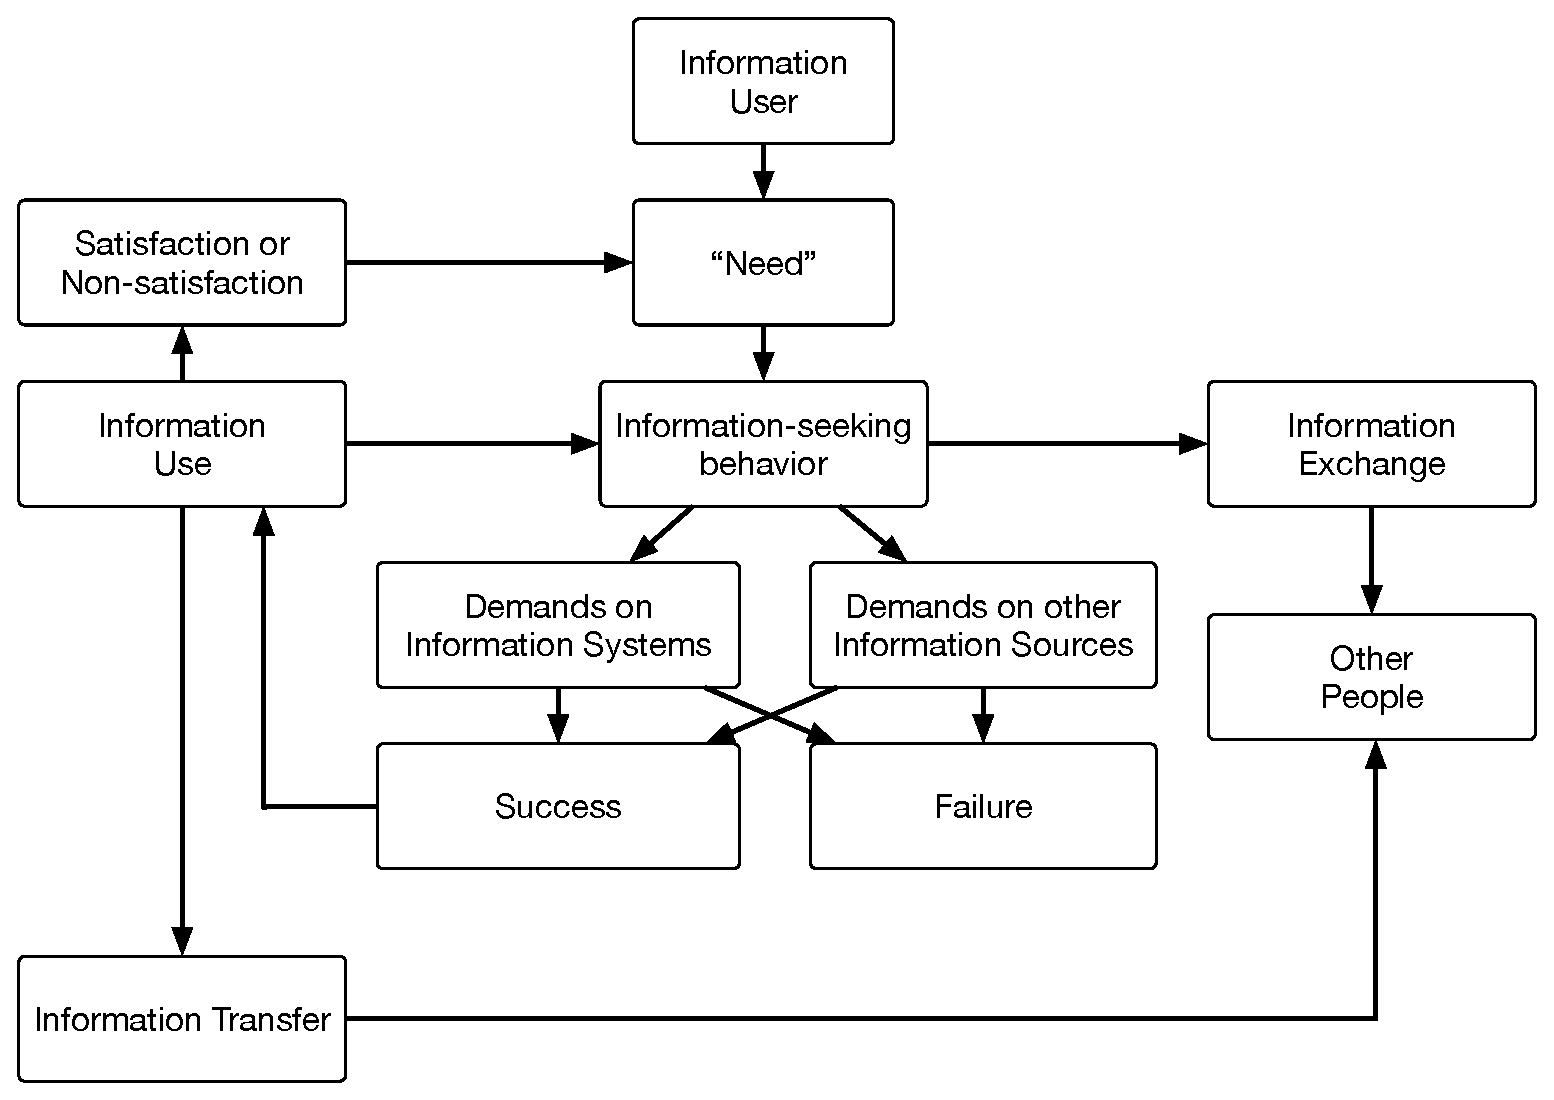
\includegraphics[width=0.7\textwidth]{figures/wilson-info-behavior}
    \caption{Wilson's information seeking behavior model \cite{wilson1981user}}
    \label{fig:wilson-info-seek}
\end{figure}

Wilson's model has been envolved many years since its origin, and it was revised and adapted to our digital world since the digital systems learns user preferences and 
changes \cite{giannini1998receiving} the way we receiving information.

David Ellis investigated \cite{ellis1989behavioural} the information seeking behavior in physical and social science \cite{ellis1993comparison}
based on grounded theory approach \cite{aceto1994grounded} and semi-structured interviews, then described \cite{ellis1997modelling} information seeking behavior through different activities rather than a single process:
starting, chaining, browsing, differentiating, monitoring, and extracting.

Starting 

TODO: explain

\subsection{Theory of Sequence to Sequence Learning}



\cleardoublepage